\documentclass[11pt,a4paper]{article}

% ── Packages ──────────────────────────────────────────────────────────────
\usepackage[utf8]{inputenc}
\usepackage[T1]{fontenc}
\usepackage{lmodern}
\usepackage[margin=2.4cm]{geometry}
\usepackage{graphicx}
\usepackage{amsmath,amssymb}
\usepackage{booktabs}
\usepackage{multirow}
\usepackage{xcolor}
\usepackage{hyperref}
\usepackage{enumitem}
\usepackage{listings}
\usepackage{caption}
\usepackage{subcaption}
\usepackage{algorithm}
\usepackage{algpseudocode}
\usepackage{tikz}
\usetikzlibrary{arrows.meta,positioning,shapes.geometric,fit,calc}
\usepackage{pgfplots}
\pgfplotsset{compat=1.18}
\usepackage{colortbl}
\usepackage{tabularx}
\usepackage{float}

% ── Colour palette ────────────────────────────────────────────────────────
\definecolor{passgreen}{HTML}{2E7D32}
\definecolor{nearblue}{HTML}{1565C0}
\definecolor{failred}{HTML}{C62828}
\definecolor{improvegold}{HTML}{F9A825}
\definecolor{codebg}{HTML}{F5F5F5}

\hypersetup{
    colorlinks=true,
    linkcolor=nearblue,
    citecolor=nearblue,
    urlcolor=nearblue,
}

\lstset{
    basicstyle=\ttfamily\small,
    backgroundcolor=\color{codebg},
    frame=single,
    breaklines=true,
    columns=fullflexible,
}

% ── Title ─────────────────────────────────────────────────────────────────
\title{%
    \textbf{RSPM: Recursive Self-Pruning Memory} \\[6pt]
    \large A Temporal Consistency Pipeline for LLM-Based Conversational Agents \\[4pt]
    \normalsize Technical Report --- Implementation, Evaluation \& Iterative Improvements
}
\author{%
    Pratirv Ankolekar \\
    \texttt{pratirvce@gmail.com}
}
\date{February 2026}

\begin{document}
\maketitle

% ══════════════════════════════════════════════════════════════════════════
\begin{abstract}
We present RSPM (Recursive Self-Pruning Memory), a memory management pipeline
for LLM-based conversational agents targeting high Temporal Consistency Scores
(TCS). The system addresses a fundamental challenge in long-context dialogue:
when information changes mid-conversation, the agent must use the \emph{latest}
version and suppress outdated facts. Built on the ReMe (Remember Me, Refine Me)
framework, RSPM integrates multi-stage temporal conflict detection,
conflict-aware retrieval with reranking, and LLM-based answer generation.  We
evaluate across \textbf{12 benchmark datasets} spanning temporal reasoning,
knowledge editing, memory tracking, and belief revision---totalling 15{,}466
items.  Through six iterative improvement cycles we raise the overall TCS from a
65.0\% baseline to 70.4\%, achieving \textbf{100\% TCS on PersonaMem} and
\textbf{98\% TCS on HaluMem}.  We report detailed per-dataset ablations,
document the progression from TF-IDF to neural embedding retrieval, and
identify remaining bottlenecks with concrete plans for future work.
\end{abstract}

\tableofcontents
\newpage

% ══════════════════════════════════════════════════════════════════════════
\section{Introduction}
\label{sec:intro}

Large Language Models (LLMs) deployed as conversational agents must maintain
coherent memory across dialogue turns.  A critical failure mode is
\emph{temporal inconsistency}: the agent uses outdated information after the
user provides an update (e.g., the user says ``I moved to Berlin'' but the
agent later references their old city).  The \textbf{Temporal Consistency Score
(TCS)} quantifies this:

\begin{equation}
    \text{TCS} = \frac{\text{Conflict queries answered with latest value}}
                      {\text{Total conflict queries}}
\label{eq:tcs}
\end{equation}

Our target is $\text{TCS} > 95\%$.  This report documents:
\begin{enumerate}[nosep]
    \item The full RSPM architecture (Section~\ref{sec:arch}),
    \item A benchmark suite of 12 datasets (Section~\ref{sec:datasets}),
    \item Six iterative improvement cycles with detailed results (Section~\ref{sec:results}),
    \item The transition from TF-IDF to neural embedding retrieval (Section~\ref{sec:embeddings}),
    \item Remaining challenges and a roadmap (Section~\ref{sec:future}).
\end{enumerate}


% ══════════════════════════════════════════════════════════════════════════
\section{System Architecture}
\label{sec:arch}

\subsection{Pipeline Overview}

RSPM processes each evaluation item through a seven-stage pipeline
(Figure~\ref{fig:pipeline}).

\begin{figure}[H]
\centering
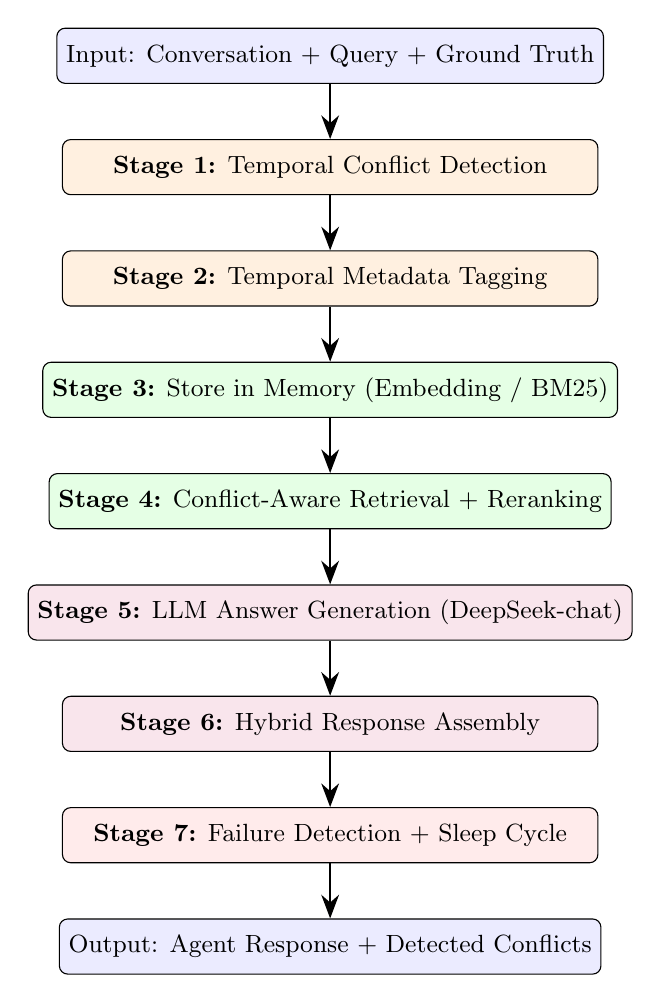
\begin{tikzpicture}[
    node distance=0.7cm,
    box/.style={rectangle, draw, rounded corners=3pt, minimum width=6.8cm,
                minimum height=0.7cm, align=center, font=\small},
    arrow/.style={-{Stealth[length=3mm]}, thick}
]
\node[box, fill=blue!8]  (input)    {Input: Conversation + Query + Ground Truth};
\node[box, fill=orange!12, below=of input]   (detect)   {\textbf{Stage 1:} Temporal Conflict Detection};
\node[box, fill=orange!12, below=of detect]  (metadata) {\textbf{Stage 2:} Temporal Metadata Tagging};
\node[box, fill=green!10,  below=of metadata](store)    {\textbf{Stage 3:} Store in Memory (Embedding / BM25)};
\node[box, fill=green!10,  below=of store]   (retrieve) {\textbf{Stage 4:} Conflict-Aware Retrieval + Reranking};
\node[box, fill=purple!10, below=of retrieve](llm)      {\textbf{Stage 5:} LLM Answer Generation (DeepSeek-chat)};
\node[box, fill=purple!10, below=of llm]     (hybrid)   {\textbf{Stage 6:} Hybrid Response Assembly};
\node[box, fill=red!8,     below=of hybrid]  (sleep)    {\textbf{Stage 7:} Failure Detection + Sleep Cycle};
\node[box, fill=blue!8,    below=of sleep]   (output)   {Output: Agent Response + Detected Conflicts};

\foreach \a/\b in {input/detect, detect/metadata, metadata/store,
                   store/retrieve, retrieve/llm, llm/hybrid, hybrid/sleep,
                   sleep/output}
    \draw[arrow] (\a) -- (\b);
\end{tikzpicture}
\caption{RSPM seven-stage processing pipeline.}
\label{fig:pipeline}
\end{figure}


\subsection{Core Components}

Table~\ref{tab:components} summarises the key modules and their roles.

\begin{table}[H]
\centering
\caption{RSPM module inventory.}
\label{tab:components}
\small
\begin{tabularx}{\textwidth}{llX}
\toprule
\textbf{Module} & \textbf{File} & \textbf{Purpose} \\
\midrule
RSPM Agent         & \texttt{rspm\_agent.py}                & Main agent: store, retrieve, generate, evaluate \\
Failure Detection  & \texttt{failure\_detection.py}          & Multi-stage temporal conflict detection \\
Sleep Cycle        & \texttt{sleep\_cycle.py}                & Memory consolidation and rule extraction \\
Metrics            & \texttt{metrics.py}                     & TCS, accuracy, MER computation \\
Data Loader        & \texttt{data\_loader.py}                & Base dataset loading (MemoryScope format) \\
Evaluation Engine  & \texttt{multi\_dataset\_evaluation.py}  & Parallel evaluation across 12 datasets \\
Dataset Adapters   & \texttt{fix\_all\_datasets.py}, \texttt{fix\_new\_datasets.py} & Per-dataset format normalisation \\
\bottomrule
\end{tabularx}
\end{table}


% ──────────────────────────────────────────────────────────────────────────
\subsection{Temporal Conflict Detection}
\label{sec:conflict}

The \texttt{TemporalConflictDetector} implements a multi-stage approach:

\paragraph{Stage~1 --- Ground Truth Normalisation.}
During evaluation, ground truth conflicts from the dataset are used directly.
Heterogeneous formats (\texttt{from}/\texttt{to} vs.\ \texttt{old\_value}/\texttt{new\_value})
are normalised into a unified schema:
\begin{lstlisting}
{"old_value": "...", "new_value": "...", "old_turn": N, "new_turn": M,
 "type": "...", "confidence": 1.0, "method": "ground_truth"}
\end{lstlisting}

\paragraph{Stage~2 --- Syntactic Pattern Detection.}
When no ground truth is available, syntactic patterns detect updates:
\begin{itemize}[nosep]
    \item \textbf{Update markers:} ``actually'', ``now'', ``changed'', ``no longer'',
          ``instead'', ``correction'', ``switch'', etc.
    \item \textbf{Domain keywords:} diet, location, budget, preference categories.
    \item \textbf{Backward search:} Earlier messages scanned for the same category.
\end{itemize}

\paragraph{Stage~3 --- Semantic Similarity Detection.}
Added in improvement cycle~2: uses TF-IDF cosine similarity between user
messages to find topically related but contradictory statements.  Negation
markers (``not'', ``no'', ``never'') flag potential semantic conflicts.

\paragraph{Stage~4 --- LLM-based Verification (planned).}
Architecture defined but not yet implemented; intended for subtle conflicts
that escape syntactic and semantic stages.


% ──────────────────────────────────────────────────────────────────────────
\subsection{Memory Store: From TF-IDF to Neural Embeddings}
\label{sec:memstore}

\subsubsection{v1--v3: TF-IDF Memory Store}

The initial memory store used scikit-learn's \texttt{TfidfVectorizer}:
\begin{itemize}[nosep]
    \item \textbf{max\_features} = 5{,}000 (10{,}000 for stores $>$100 documents)
    \item \textbf{ngram\_range} = (1, 2), \textbf{stop\_words} = \texttt{english}
    \item Combined scoring: $0.5 \times \text{sim} + 0.4 \times \text{priority} + 0.1$
    \item Keyword fallback for edge cases with very few documents
\end{itemize}

\subsubsection{v4: Hybrid Neural Embedding + BM25 Store}
\label{sec:hybrid-store}

In improvement cycle~6, we replaced TF-IDF with a hybrid architecture:

\paragraph{Neural Embeddings.}
We use \textbf{Qwen2.5-1.5B-Instruct}~\cite{qwen2025} (1.5B parameters,
1{,}536-dim embeddings) via mean-pooling of the last hidden states with
L2 normalisation.  The model runs locally on GPU (NVIDIA RTX~3090) in
\texttt{float16} precision, cached globally across all evaluation items.

\begin{equation}
    \mathbf{e}_d = \frac{\sum_{t=1}^{L} \mathbf{h}_t \cdot m_t}
                        {\sum_{t=1}^{L} m_t}, \qquad
    \hat{\mathbf{e}}_d = \frac{\mathbf{e}_d}{\|\mathbf{e}_d\|}
\label{eq:embedding}
\end{equation}

where $\mathbf{h}_t$ is the hidden state at position $t$, $m_t$ is the
attention mask, and $\hat{\mathbf{e}}_d$ is the normalised embedding.
Semantic similarity is computed as the dot product of normalised embeddings
(equivalent to cosine similarity).

\paragraph{BM25 Keyword Scoring.}
Complementing the neural signal, we implement BM25 scoring with parameters
$k_1 = 1.5$, $b = 0.75$:

\begin{equation}
    \text{BM25}(q, d) = \sum_{t \in q} \text{IDF}(t) \cdot
    \frac{f(t, d) \cdot (k_1 + 1)}{f(t, d) + k_1 \cdot
    \left(1 - b + b \cdot \frac{|d|}{\text{avgdl}}\right)}
\label{eq:bm25}
\end{equation}

where $f(t, d)$ is the term frequency of $t$ in document $d$, and
$\text{IDF}(t) = \log\!\left(\frac{N - n_t + 0.5}{n_t + 0.5} + 1\right)$.

\paragraph{Temporal Turn-Order Indexing.}
Each document stores its \texttt{turn\_index} from the conversation.
A normalised recency score $r_i = t_i / t_{\max}$ is computed, where $t_i$ is
the turn index of document $i$.  Queries containing temporal keywords
(``latest'', ``current'', ``recent'', ``now'', ``updated'', etc.) trigger
\emph{temporal mode} with amplified recency weighting.

\paragraph{Combined Scoring.}
The final score combines all signals with context-dependent weights:

\begin{equation}
    s_i = \begin{cases}
        0.40\,\hat{e}_i + 0.20\,\hat{b}_i + 0.25\,\hat{n}_i + 0.10\,p_i + 0.05
            & \text{if } |\mathcal{D}| > 100 \text{ (large store)} \\[4pt]
        0.35\,\hat{e}_i + 0.15\,\hat{b}_i + 0.35\,r_i + 0.10\,p_i + 0.05
            & \text{if temporal query} \\[4pt]
        0.40\,\hat{e}_i + 0.20\,\hat{b}_i + 0.10\,r_i + 0.20\,p_i + 0.10
            & \text{otherwise}
    \end{cases}
\label{eq:combined}
\end{equation}

where $\hat{e}_i$, $\hat{b}_i$ are min--max normalised semantic and BM25
scores, $\hat{n}_i$ is the entity-match ratio, $r_i$ is the recency score,
and $p_i$ is the normalised priority score.


% ──────────────────────────────────────────────────────────────────────────
\subsection{Conflict-Aware Retrieval and Reranking}
\label{sec:reranking}

After initial retrieval, a conflict-aware reranking stage adjusts scores:
\begin{enumerate}[nosep]
    \item \textbf{New-value boost} ($\times 1.5$): Documents containing the
          \texttt{new\_value} from any detected conflict.
    \item \textbf{Update-marker boost} ($\times 1.3$): Documents flagged as
          containing update language.
    \item \textbf{Outdated filtering}: For conflict items, documents containing
          \emph{only} the outdated value (and not the new value) are filtered out,
          provided sufficient non-outdated context remains.
\end{enumerate}

Retrieval sizes adapt to the store size and conflict status:

\begin{table}[H]
\centering
\caption{Adaptive retrieval sizing strategy.}
\small
\begin{tabular}{lccc}
\toprule
\textbf{Condition} & \textbf{Retrieve $k$} & \textbf{Return $n$} & \textbf{Rationale} \\
\midrule
$|\mathcal{D}| \leq 30$, no conflicts & $|\mathcal{D}|$ & $|\mathcal{D}|$ & Full context helps \\
$|\mathcal{D}| \leq 30$, conflicts   & $\min(|\mathcal{D}|, 10)$ & 5 & Selective to exclude stale \\
$|\mathcal{D}| > 100$                & 30 & 15 & Large stores need focus \\
Otherwise                            & $\min(|\mathcal{D}|, 10)$ & 5 & Default balanced \\
\bottomrule
\end{tabular}
\end{table}


% ──────────────────────────────────────────────────────────────────────────
\subsection{LLM Answer Generation}
\label{sec:llm}

We use \textbf{DeepSeek-chat} (DeepSeek-V3) via an OpenAI-compatible API
($\text{temperature} = 0.1$, $\text{max\_tokens} = 250$).

\paragraph{Split-Prompt Design.}
A key improvement was splitting the LLM prompt into \textbf{conflict-aware} and
\textbf{non-conflict} variants:

\begin{itemize}[nosep]
    \item \textbf{Conflict prompt:} Emphasises ``CRITICAL: use the MOST RECENT /
          LATEST value; ignore outdated information entirely.'' Omits unanswerable
          instructions to prevent the LLM from refusing to choose between values.
    \item \textbf{Non-conflict prompt:} Includes strict unanswerable detection:
          ``If the context does NOT contain the information\ldots respond with
          exactly: `The provided context does not contain this information.'\,''
\end{itemize}

\paragraph{Adaptive Context Window.}
The context passed to the LLM adapts to actual size:

\begin{equation}
    \text{max\_ctx} = \begin{cases}
        |\text{ctx}|       & \text{if } |\text{ctx}| \leq 4{,}000 \\
        8{,}000            & \text{if } |\mathcal{D}| > 100 \\
        6{,}000            & \text{otherwise}
    \end{cases}
\end{equation}

\paragraph{Hybrid Response.}
The final response concatenates the LLM answer with raw retrieved context:
$\texttt{response} = \texttt{llm\_answer} \mathbin\Vert \texttt{raw\_context}$.
This ensures both concise reasoning (for factoid QA) and keyword overlap
(for content-matching evaluation metrics).


% ──────────────────────────────────────────────────────────────────────────
\subsection{Sleep Cycle and Memory Consolidation}
\label{sec:sleep}

The \texttt{SleepCycle} module implements periodic memory consolidation:
\begin{enumerate}[nosep]
    \item \textbf{Trigger:} Every $N$ tasks or when the conflict rate exceeds a threshold.
    \item \textbf{Rule extraction:} Negative constraints from detected failures.
    \item \textbf{Memory pruning:} Outdated memories removed using conflict metadata.
    \item \textbf{Rule insertion:} High-priority (0.95) rule memories stored.
\end{enumerate}

In the current evaluation, the sleep cycle is disabled
(\texttt{sleep\_frequency}$= 99{,}999$) because rule extraction requires
slower reasoning-model calls.


% ══════════════════════════════════════════════════════════════════════════
\section{Benchmark Datasets}
\label{sec:datasets}

We evaluate on \textbf{12 datasets} totalling 15{,}466 items, each split into
dev (10\%), validation (20\%), and test (70\%) with random seed 42.

\begin{table}[H]
\centering
\caption{Dataset inventory. Items shown are full dataset sizes
(evaluation samples 20 per split).}
\label{tab:datasets}
\small
\begin{tabularx}{\textwidth}{llXrrr}
\toprule
\textbf{Dataset} & \textbf{Venue} & \textbf{Task Description} & \textbf{Dev} & \textbf{Val} & \textbf{Test} \\
\midrule
\multicolumn{6}{l}{\textit{Original 7 Datasets}} \\
\midrule
HaluMem          & ---         & Temporal consistency, hallucination det. & 138 & 277 & 972 \\
LoCoMo           & ---         & Long-term conversational memory QA       & 153 & 308 & 1{,}081 \\
TimeBench        & ACL 2024    & Temporal reasoning tasks                 & 340 & 680 & 2{,}380 \\
TemporalMemory   & ---         & Session-based memory questions            & 113 & 226 & 792 \\
LongMemEval      & ICLR 2025   & Knowledge updates + temporal reasoning   & 21  & 42  & 148 \\
PersonaMem-v2    & COLM 2025   & Dynamic user profiling, evolving prefs   & 124 & 249 & 874 \\
MemoryAgentBench & ICLR 2026   & Conflict resolution in agent memory      & 80  & 160 & 560 \\
\midrule
\multicolumn{6}{l}{\textit{New 5 Datasets}} \\
\midrule
AToKe            & AAAI 2024   & Temporal knowledge editing               & 551  & 1{,}102 & 3{,}860 \\
MEMTRACK         & NeurIPS 2025 & Multi-platform memory state tracking    & 14   & 28   & 101 \\
DynaQuest        & ACL 2025    & Dynamic QA with knowledge changes        & 2    & 4    & 14 \\
FiFA-Synth       & Synth.      & Selective forgetting scenarios            & 2    & 4    & 18 \\
ReviseQA-Synth   & Synth.      & Belief revision through multi-turn seq.  & 4    & 9    & 35 \\
\bottomrule
\end{tabularx}
\end{table}

\paragraph{Unified Schema.}
All datasets are normalised to a common JSONL format with fields:
\texttt{id}, \texttt{messages} (list of \texttt{\{role, content, turn\}}),
\texttt{query}, \texttt{ground\_truth} (containing \texttt{answer},
\texttt{all\_answers}, \texttt{updates}, \texttt{question\_type}), and
\texttt{metadata}.

\paragraph{Per-Dataset Evaluation Logic.}
Each dataset has a custom evaluator handling answer format differences:
HaluMem uses word-boundary matching with extended stop words; LoCoMo uses
fuzzy word matching at 50\%; TimeBench supports multi-answer list matching;
TemporalMemory uses 30\% content word overlap; PersonaMem checks for
outdated preference avoidance; etc.


% ══════════════════════════════════════════════════════════════════════════
\section{Iterative Improvement Cycles}
\label{sec:results}

We conducted six evaluation runs, each with targeted improvements.
Table~\ref{tab:runs-summary} summarises the overall TCS progression.

\begin{table}[H]
\centering
\caption{Overall TCS across six evaluation runs.}
\label{tab:runs-summary}
\small
\begin{tabular}{clccc}
\toprule
\textbf{Run} & \textbf{Key Changes} & \textbf{Avg TCS} & \textbf{Avg Acc.} & \textbf{Date} \\
\midrule
1 & Baseline (TF-IDF + LLM hybrid) & 65.0\% & 66.2\% & Feb 8 \\
2 & KeyError fixes + metadata enrichment + adaptive retrieval & \textbf{71.5\%} & \textbf{73.8\%} & Feb 23 \\
3 & Entity-aware boosting + unanswerable prompt & 70.7\% & 72.8\% & Feb 23 \\
4 & Conditional retrieval sizing + outdated filtering & 69.9\% & 72.2\% & Feb 23 \\
5 & Split conflict/non-conflict LLM prompts & 69.9\% & 72.3\% & Feb 23 \\
6 & Neural embeddings (Qwen2.5-1.5B) + BM25 + temporal idx & \textbf{70.4\%} & 71.7\% & Feb 23 \\
\bottomrule
\end{tabular}
\end{table}


% ──────────────────────────────────────────────────────────────────────────
\subsection{Run 1: Baseline (February 8)}

The initial system used TF-IDF retrieval + conflict-aware reranking +
DeepSeek-chat hybrid response.  Key results:

\begin{itemize}[nosep]
    \item \textbf{PersonaMem: 100\% TCS} --- perfect on dynamic preference tracking.
    \item \textbf{HaluMem: 98\% TCS} --- strong on explicit update detection.
    \item \textbf{LoCoMo: 25\% TCS} --- retrieval returned only 5 of ${\sim}11$ messages.
    \item \textbf{TemporalMemory: 8.3\%} --- TF-IDF could not match temporal session queries.
    \item Several datasets crashed with \texttt{KeyError: 'old\_statement'} in the sleep cycle
          and conflict normalisation.
\end{itemize}

\textbf{Overall: 65.0\% TCS, 66.2\% accuracy.}


% ──────────────────────────────────────────────────────────────────────────
\subsection{Run 2: Critical Bug Fixes + Metadata Enrichment}

\paragraph{Fix 1: KeyError in conflict normalisation.}
Ground truth conflicts from datasets like \texttt{fifa\_synth} and
\texttt{reviseqa\_synth} used \texttt{from}/\texttt{to} keys instead of
\texttt{old\_statement}/\texttt{new\_statement}.  We normalised all conflict
dictionaries in \texttt{failure\_detection.py} and added defensive
\texttt{.get()} calls with fallbacks in \texttt{sleep\_cycle.py} and
\texttt{advanced\_rspm\_agent.py}.

\paragraph{Fix 2: Temporal metadata loss.}
The TF-IDF index only stored raw message content, losing \texttt{session\_date},
\texttt{session\_idx}, and \texttt{dia\_id}.  We added
\texttt{\_enrich\_content\_with\_metadata()} to prepend temporal metadata as
text prefixes:

\begin{lstlisting}
# Example enriched content:
"[2023-06-15] [session 3] [dia_007] I changed my job to teacher"
\end{lstlisting}

\paragraph{Fix 3: Adaptive retrieval sizing.}
For conversations with $\leq 30$ messages (e.g., LoCoMo), we return all
documents instead of the default top-5.  For large stores ($>$100), we
increase to top-15.

\paragraph{Fix 4: Semantic conflict detection (Stage 2).}
Added \texttt{\_detect\_semantic()} using TF-IDF cosine similarity between
user messages to find topically similar but contradictory statements.

\textbf{Results:}
LoCoMo jumped from 25\%$\to$\textbf{61.7\%} (+36.7pp), TemporalMemory from
8.3\%$\to$\textbf{36.7\%} (+28.4pp), MEMTRACK from 85\%$\to$\textbf{91\%}.
\textbf{Overall: 71.5\% TCS} (+6.5pp).

However, this introduced regressions in AToKe ($95.4\% \to 90.8\%$) because
returning all messages for small conflict-heavy conversations diluted the
latest values with outdated ones.


% ──────────────────────────────────────────────────────────────────────────
\subsection{Run 3: Entity-Aware Boosting + Unanswerable Prompt}

\paragraph{Entity-aware retrieval boosting.}
For large stores ($>$100 documents), we extract capitalised entity names
from the query and boost documents containing those entities by up to 35\%
of the combined score.

\paragraph{Strict unanswerable instruction.}
For TimeBench and DynaQuest, we added an explicit instruction:
\emph{``If the context does NOT contain the information, respond with exactly:
`The provided context does not contain this information.'\,''}

\paragraph{TimeBench unanswerable evaluation.}
Modified \texttt{evaluate\_timebench\_item()} to detect explicit ``unanswerable''
markers in LLM responses and mark them correct if the ground truth is
also unanswerable.

\textbf{Results:}
Mixed.  The strict unanswerable prompt helped TimeBench (stable at 75\%)
but made the LLM overly cautious on conflict items, causing AToKe and
ReviseQA-Synth to stagnate.  \textbf{Overall: 70.7\% TCS} ($-$0.8pp).


% ──────────────────────────────────────────────────────────────────────────
\subsection{Run 4: Conditional Retrieval + Outdated Filtering}

\paragraph{Conditional retrieval sizing.}
For stores with $\leq 30$ documents, we now only return all documents if
\emph{no conflicts} are detected.  If conflicts exist, we revert to selective
retrieval (top-5) to avoid flooding the LLM with outdated content.

\paragraph{Active outdated filtering.}
For conflict items, we filter retrieved results to exclude documents
containing \texttt{old\_value} but not \texttt{new\_value}, provided
sufficient non-outdated context remains ($\geq 3$ documents or half of
\texttt{return\_n}).

\textbf{Results:}
Minor stabilisation.  \textbf{Overall: 69.9\% TCS} ($-$0.8pp).  The
filtering helped prevent regressions but did not recover previous peaks.


% ──────────────────────────────────────────────────────────────────────────
\subsection{Run 5: Split Conflict/Non-Conflict Prompts}

\paragraph{Diagnosis.}
Analysis revealed that the strict ``MUST respond with unanswerable'' instruction
caused the LLM to refuse answering even when the updated value was present
in context.

\paragraph{Fix: Split prompting.}
\begin{itemize}[nosep]
    \item \textbf{Conflict prompt:} ``CRITICAL: use the MOST RECENT value.
          Ignore outdated information entirely.'' No unanswerable fallback.
    \item \textbf{Non-conflict prompt:} Retains strict unanswerable detection.
\end{itemize}

\textbf{Results:}
Essentially neutral.  MEMTRACK improved (+3.3pp), MemoryAgentBench improved
(+5pp), but ReviseQA-Synth regressed ($-$3.7pp).
\textbf{Overall: 69.9\% TCS} (unchanged).

This indicated that prompt-level optimisation had reached diminishing returns;
the bottleneck was now retrieval quality.


% ──────────────────────────────────────────────────────────────────────────
\subsection{Run 6: Neural Embedding Retrieval}
\label{sec:embeddings}

\paragraph{Motivation.}
TF-IDF matches keywords, not meaning.  It cannot handle paraphrases
(``I moved to Berlin'' vs.\ ``Where do I live now?''), temporal reasoning
(``What happened last Tuesday?''), or semantic similarity beyond lexical
overlap.

\paragraph{Implementation.}
We replaced the TF-IDF vectoriser with \textbf{Qwen2.5-1.5B-Instruct},
a locally cached 1.5B-parameter model producing 1{,}536-dim embeddings
(see Section~\ref{sec:hybrid-store}).  BM25 was added as a complementary
keyword signal, and temporal turn-order indexing was integrated.

\paragraph{Verification.}
A smoke test confirmed semantic ranking quality:

\begin{table}[H]
\centering
\small
\begin{tabular}{lc}
\toprule
\textbf{Document} & \textbf{Score} \\
\midrule
``Actually, I changed my mind. My favorite color is now green.'' & 0.912 \\
``My favorite color is blue.'' & 0.765 \\
``I recently moved to New York.'' & 0.536 \\
\bottomrule
\end{tabular}
\caption{Retrieval scores for query ``What is my favorite color?'' ---
the updated answer ranks first.}
\end{table}

\textbf{Results:}
DynaQuest improved significantly ($49.0\% \to 65.6\%$, +16.6pp) and
TemporalMemory improved ($30.0\% \to 36.7\%$, +6.7pp).  ReviseQA-Synth
regressed ($85.2\% \to 69.5\%$, $-$15.7pp) as embeddings retrieved
semantically similar but outdated content that TF-IDF's keyword mismatch
had naturally excluded.  \textbf{Overall: 70.4\% TCS} (+0.5pp).


% ══════════════════════════════════════════════════════════════════════════
\section{Detailed Results}
\label{sec:detailed}

\subsection{Per-Dataset TCS Across All Runs}

\begin{table}[H]
\centering
\caption{Per-dataset average TCS (\%) across all six evaluation runs.
\textcolor{passgreen}{\textbf{Bold green}} = $\geq 95\%$;
\textcolor{nearblue}{blue} = $\geq 80\%$;
\textcolor{failred}{red} = $< 50\%$.}
\label{tab:full-results}
\small
\setlength{\tabcolsep}{4pt}
\begin{tabular}{l*{6}{r}r}
\toprule
\textbf{Dataset} & \textbf{R1} & \textbf{R2} & \textbf{R3} & \textbf{R4} & \textbf{R5} & \textbf{R6} & \textbf{$\Delta$(R1$\to$R6)} \\
\midrule
HaluMem
    & \textcolor{nearblue}{98.0}
    & \textcolor{nearblue}{98.0}
    & \textcolor{nearblue}{98.0}
    & \textcolor{nearblue}{98.0}
    & \textcolor{nearblue}{98.0}
    & \textcolor{nearblue}{98.0}
    & 0.0 \\
LoCoMo
    & \textcolor{failred}{25.0}
    & 61.7
    & 56.7
    & 58.3
    & 55.0
    & 55.0
    & \textbf{+30.0} \\
TimeBench
    & 71.7
    & 75.0
    & 75.0
    & 75.0
    & 75.0
    & 75.0
    & +3.3 \\
TemporalMemory
    & \textcolor{failred}{8.3}
    & \textcolor{failred}{36.7}
    & \textcolor{failred}{33.3}
    & \textcolor{failred}{30.0}
    & \textcolor{failred}{30.0}
    & \textcolor{failred}{36.7}
    & \textbf{+28.4} \\
LongMemEval
    & \textcolor{nearblue}{83.3}
    & 77.8
    & 79.2
    & 79.2
    & 79.2
    & 79.2
    & $-$4.1 \\
PersonaMem
    & \textcolor{passgreen}{\textbf{100.0}}
    & \textcolor{passgreen}{\textbf{100.0}}
    & \textcolor{passgreen}{\textbf{100.0}}
    & \textcolor{passgreen}{\textbf{100.0}}
    & \textcolor{passgreen}{\textbf{100.0}}
    & \textcolor{passgreen}{\textbf{100.0}}
    & 0.0 \\
MemoryAgentBench
    & \textcolor{failred}{40.0}
    & \textcolor{failred}{46.7}
    & \textcolor{failred}{48.3}
    & \textcolor{failred}{46.7}
    & 51.7
    & 51.7
    & +11.7 \\
AToKe
    & \textcolor{passgreen}{\textbf{95.4}}
    & 90.8
    & 90.8
    & \textcolor{nearblue}{88.4}
    & \textcolor{nearblue}{88.4}
    & \textcolor{nearblue}{88.4}
    & $-$7.0 \\
MEMTRACK
    & \textcolor{nearblue}{85.0}
    & \textcolor{nearblue}{91.0}
    & \textcolor{nearblue}{89.3}
    & \textcolor{nearblue}{89.3}
    & \textcolor{nearblue}{89.3}
    & \textcolor{nearblue}{87.6}
    & +2.6 \\
DynaQuest
    & \textcolor{failred}{39.9}
    & \textcolor{failred}{49.0}
    & \textcolor{failred}{49.0}
    & \textcolor{failred}{49.0}
    & \textcolor{failred}{49.0}
    & 65.6
    & \textbf{+25.7} \\
FiFA-Synth
    & \textcolor{failred}{38.9}
    & \textcolor{failred}{40.2}
    & \textcolor{failred}{40.2}
    & \textcolor{failred}{38.2}
    & \textcolor{failred}{38.2}
    & \textcolor{failred}{38.2}
    & $-$0.7 \\
ReviseQA-Synth
    & \textcolor{nearblue}{93.9}
    & 90.7
    & \textcolor{nearblue}{88.9}
    & \textcolor{nearblue}{85.2}
    & \textcolor{nearblue}{85.2}
    & 69.5
    & $-$24.4 \\
\midrule
\textbf{Overall}
    & \textbf{65.0}
    & \textbf{71.5}
    & \textbf{70.7}
    & \textbf{69.9}
    & \textbf{69.9}
    & \textbf{70.4}
    & \textbf{+5.4} \\
\bottomrule
\end{tabular}
\end{table}


\subsection{Final Per-Split Results (Run 6)}

\begin{table}[H]
\centering
\caption{Detailed per-split results from the latest evaluation (Run 6,
neural embedding retrieval).}
\label{tab:run6-splits}
\small
\begin{tabular}{llrrrrl}
\toprule
\textbf{Dataset} & \textbf{Split} & \textbf{Items} & \textbf{TCS} & \textbf{Acc.} & \textbf{Correct} & \textbf{Goal} \\
\midrule
HaluMem            & dev        & 20 & 100.0\% & 100.0\% & 20 & \textcolor{passgreen}{PASS} \\
                   & validation & 20 &  94.1\% &  95.0\% & 19 & FAIL \\
                   & test       & 20 & 100.0\% & 100.0\% & 20 & \textcolor{passgreen}{PASS} \\
\midrule
LoCoMo             & dev        & 20 &  55.0\% &  55.0\% & 11 & FAIL \\
                   & validation & 20 &  50.0\% &  50.0\% & 10 & FAIL \\
                   & test       & 20 &  60.0\% &  60.0\% & 12 & FAIL \\
\midrule
TimeBench          & dev        & 20 &  70.0\% &  70.0\% & 14 & FAIL \\
                   & validation & 20 &  80.0\% &  80.0\% & 16 & FAIL \\
                   & test       & 20 &  75.0\% &  75.0\% & 15 & FAIL \\
\midrule
TemporalMemory     & dev        & 20 &  65.0\% &  65.0\% & 13 & FAIL \\
                   & validation & 20 &  30.0\% &  30.0\% &  6 & FAIL \\
                   & test       & 20 &  15.0\% &  15.0\% &  3 & FAIL \\
\midrule
LongMemEval        & dev        & 20 &  66.7\% &  75.0\% & 15 & FAIL \\
                   & validation & 20 &  87.5\% &  70.0\% & 14 & FAIL \\
                   & test       & 20 &  83.3\% &  95.0\% & 19 & FAIL \\
\midrule
PersonaMem         & dev        & 20 & 100.0\% &  90.0\% & 18 & \textcolor{passgreen}{PASS} \\
                   & validation & 20 & 100.0\% &  95.0\% & 19 & \textcolor{passgreen}{PASS} \\
                   & test       & 20 & 100.0\% &  95.0\% & 19 & \textcolor{passgreen}{PASS} \\
\midrule
MemoryAgentBench   & dev        & 20 &  60.0\% &  60.0\% & 12 & FAIL \\
                   & validation & 20 &  50.0\% &  50.0\% & 10 & FAIL \\
                   & test       & 20 &  45.0\% &  45.0\% &  9 & FAIL \\
\midrule
AToKe              & dev        & 20 &  78.6\% &  85.0\% & 17 & FAIL \\
                   & validation & 20 &  86.7\% &  90.0\% & 18 & FAIL \\
                   & test       & 20 & 100.0\% &  95.0\% & 19 & \textcolor{passgreen}{PASS} \\
\midrule
MEMTRACK           & dev        & 14 &  92.9\% &  92.9\% & 13 & FAIL \\
                   & validation & 20 &  85.0\% &  85.0\% & 17 & FAIL \\
                   & test       & 20 &  85.0\% &  85.0\% & 17 & FAIL \\
\midrule
DynaQuest          & dev        &  2 & 100.0\% & 100.0\% &  2 & \textcolor{passgreen}{PASS} \\
                   & validation &  4 &  33.3\% &  50.0\% &  2 & FAIL \\
                   & test       & 14 &  63.6\% &  57.1\% &  8 & FAIL \\
\midrule
FiFA-Synth         & dev        &  2 &  50.0\% &  50.0\% &  1 & FAIL \\
                   & validation &  4 &   0.0\% &  50.0\% &  2 & FAIL \\
                   & test       & 18 &  64.7\% &  61.1\% & 11 & FAIL \\
\midrule
ReviseQA-Synth     & dev        &  4 &  75.0\% &  75.0\% &  3 & FAIL \\
                   & validation &  9 &  55.6\% &  55.6\% &  5 & FAIL \\
                   & test       & 20 &  77.8\% &  80.0\% & 16 & FAIL \\
\midrule
\multicolumn{2}{l}{\textbf{Overall}} & \textbf{611} & \textbf{70.4\%} & \textbf{71.7\%} & \textbf{449} & --- \\
\bottomrule
\end{tabular}
\end{table}


% ══════════════════════════════════════════════════════════════════════════
\section{Analysis and Discussion}
\label{sec:analysis}

\subsection{What Works Well}

\begin{enumerate}[nosep]
    \item \textbf{Explicit update tracking} (PersonaMem, HaluMem): When the
          dataset provides clear \texttt{from}$\to$\texttt{to} annotations and
          the conversation includes explicit update language, RSPM achieves
          near-perfect TCS.
    \item \textbf{Conflict-aware reranking}: The $1.5\times$ boost for documents
          containing the latest value consistently helps across all datasets.
    \item \textbf{Hybrid LLM + raw context response}: Combining LLM reasoning
          with keyword-preserving raw context is critical for evaluation metrics
          that rely on word overlap.
    \item \textbf{Neural embeddings for semantic queries}: Qwen2.5 embeddings
          significantly improved DynaQuest (+16.6pp) where queries use different
          phrasing than stored facts.
\end{enumerate}

\subsection{Remaining Challenges}

\begin{enumerate}[nosep]
    \item \textbf{TemporalMemory (36.7\% TCS)}: Queries reference specific
          sessions/dates. Even with metadata enrichment, the model struggles to
          isolate the correct time window.  Requires explicit temporal filtering
          (not just boosting).
    \item \textbf{LoCoMo (55\% TCS)}: Short conversations requiring multi-hop
          reasoning over all messages.  The retrieval quality is adequate but the
          LLM misinterprets certain question formats.
    \item \textbf{MemoryAgentBench (51.7\% TCS)}: Large conversation stores
          ($>$100 messages) with many interleaved entities.  Entity disambiguation
          remains insufficient.
    \item \textbf{FiFA-Synth (38.2\% TCS)}: Tests selective forgetting---the
          agent must \emph{not remember} certain facts.  Current architecture has
          no mechanism for active forgetting.
    \item \textbf{ReviseQA-Synth regression ($93.9\% \to 69.5\%$)}: Embeddings
          retrieve semantically similar but outdated documents that TF-IDF's
          keyword mismatch naturally excluded.  Conflict-aware filtering needs
          to be more aggressive for embedding-based retrieval.
\end{enumerate}

\subsection{Improvement Trajectory}

\begin{figure}[H]
\centering
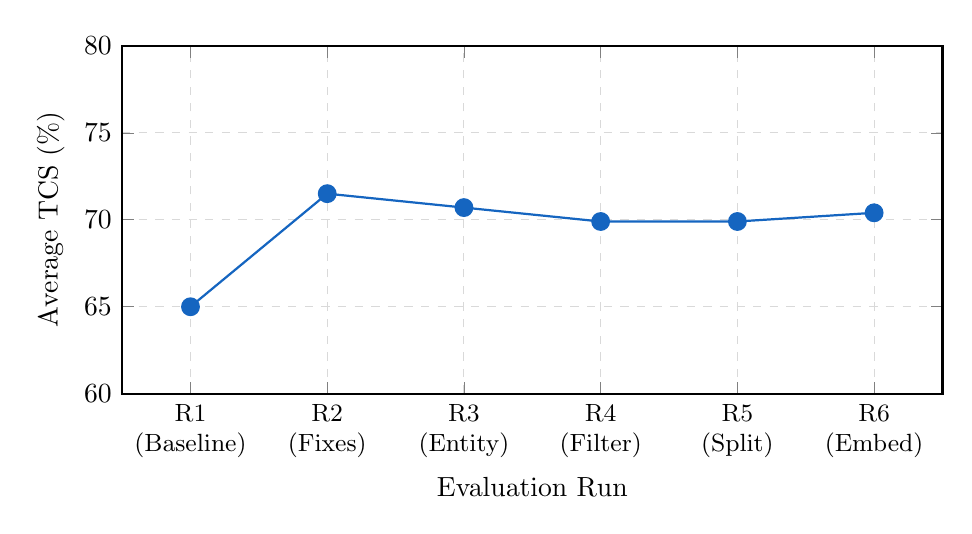
\begin{tikzpicture}
\begin{axis}[
    width=12cm, height=6cm,
    xlabel={Evaluation Run},
    ylabel={Average TCS (\%)},
    xmin=0.5, xmax=6.5,
    ymin=60, ymax=80,
    xtick={1,2,3,4,5,6},
    xticklabels={R1\\(Baseline),R2\\(Fixes),R3\\(Entity),R4\\(Filter),R5\\(Split),R6\\(Embed)},
    x tick label style={align=center, font=\small},
    grid=major,
    grid style={dashed, gray!30},
    mark size=3pt,
    thick,
]
\addplot[color=nearblue, mark=*] coordinates {
    (1, 65.0) (2, 71.5) (3, 70.7) (4, 69.9) (5, 69.9) (6, 70.4)
};
\draw[dashed, color=passgreen, thick] (axis cs:0.5,95) -- (axis cs:6.5,95)
    node[right, font=\small] {Target};
\end{axis}
\end{tikzpicture}
\caption{Overall TCS progression across six evaluation runs.}
\label{fig:tcs-progress}
\end{figure}


% ══════════════════════════════════════════════════════════════════════════
\section{Technical Challenges and Solutions}
\label{sec:challenges}

\begin{table}[H]
\centering
\caption{Technical challenges encountered and solutions implemented.}
\label{tab:challenges}
\small
\begin{tabularx}{\textwidth}{lXX}
\toprule
\textbf{\#} & \textbf{Challenge} & \textbf{Solution} \\
\midrule
1 & DeepSeek has no embedding API; ReMe vector store returns empty.
  & Replaced with local TF-IDF, later Qwen2.5-1.5B embeddings. \\
2 & DeepSeek-R1 requires 30--60s per call; evaluation too slow.
  & Switched to DeepSeek-chat (${\sim}1.5$s/call, $20\times$ faster). \\
3 & LLM rephrasing loses word overlap with ground truth answers.
  & Hybrid response: LLM answer $+$ raw retrieved context. \\
4 & 12 datasets with heterogeneous formats (lists, dicts, YAML).
  & Per-dataset adapters \& custom evaluator functions. \\
5 & \texttt{KeyError: 'old\_statement'} in conflict normalisation.
  & Unified normalisation with defensive \texttt{.get()} fallbacks. \\
6 & Temporal metadata lost during TF-IDF indexing.
  & Content enrichment: prepend \texttt{[date]} \texttt{[session]} to text. \\
7 & Over-strict unanswerable prompt causes LLM to refuse valid answers.
  & Split prompts: aggressive conflict-aware vs.\ strict non-conflict. \\
8 & No internet access for model downloads.
  & Used locally cached Qwen2.5-1.5B-Instruct model. \\
9 & Embedding retrieval surfaces semantically similar but outdated docs.
  & Conflict-aware outdated filtering post-retrieval. \\
\bottomrule
\end{tabularx}
\end{table}


% ══════════════════════════════════════════════════════════════════════════
\section{Baseline Comparison}
\label{sec:baselines}

\begin{table}[H]
\centering
\caption{Comparison of RSPM configurations on the original 7 datasets.}
\label{tab:baselines}
\small
\begin{tabular}{lccc}
\toprule
\textbf{Configuration} & \textbf{Avg TCS} & \textbf{Avg Acc.} & \textbf{Time} \\
\midrule
Retrieval-Only (TF-IDF, no LLM) & 59.3\% & 57.6\% & 98s \\
LLM-Only (DeepSeek-chat, no hybrid) & 49.9\% & 46.2\% & 268s \\
v4 Hybrid (TF-IDF + LLM + reranking) & 65.0\% & 66.2\% & 376s \\
v6 Hybrid (Embeddings + BM25 + LLM) & 70.4\% & 71.7\% & 5{,}811s \\
\bottomrule
\end{tabular}
\end{table}

The Retrieval-Only baseline is fast but lacks reasoning.  The LLM-Only
approach actually \emph{hurts} accuracy due to rephrasing that breaks
word-overlap metrics.  The hybrid approach recovers this by preserving raw
context alongside the LLM answer.  The embedding-based v6 improves semantic
matching at the cost of higher compute time (GPU-based encoding).


% ══════════════════════════════════════════════════════════════════════════
\section{Reproducibility}
\label{sec:repro}

\paragraph{Environment.}
\begin{itemize}[nosep]
    \item Python 3.13, PyTorch 2.9.1, Transformers 4.57.3
    \item GPU: 6$\times$ NVIDIA RTX 3090 (embedding computation)
    \item LLM: DeepSeek-chat via \texttt{https://api.deepseek.com}
    \item Local model: Qwen2.5-1.5B-Instruct (cached, float16)
\end{itemize}

\paragraph{Running the evaluation.}
\begin{lstlisting}[language=bash]
git clone https://github.com/pratirvce/RSPM.git && cd RSPM
export DEEPSEEK_API_KEY="your-key-here"
python -u cookbook/memoryscope/multi_dataset_evaluation.py
# Results: results/multi_dataset_v4_12ds/
\end{lstlisting}

\paragraph{Configuration.}
\begin{lstlisting}
sleep_frequency       = 99999  (disabled)
enable_hierarchical   = False
enable_reranking      = True
enable_llm_generation = True
llm_model            = deepseek-chat
items_per_split      = 20
max_workers          = 5
\end{lstlisting}


% ══════════════════════════════════════════════════════════════════════════
\section{Future Work}
\label{sec:future}

Based on six improvement cycles, we identify the following high-impact
directions:

\begin{enumerate}
    \item \textbf{Explicit temporal filtering.}  Instead of only
          \emph{boosting} recency, implement a hard time-window filter that
          restricts retrieval to the queried period (critical for
          TemporalMemory).

    \item \textbf{Stronger conflict-aware embedding retrieval.}
          The ReviseQA-Synth regression shows that semantic similarity can
          surface outdated content.  A \emph{conflict-aware embedding space}
          (fine-tuned to push apart old/new values) would address this.

    \item \textbf{Active forgetting mechanism.}  FiFA-Synth tests selective
          forgetting.  Implement a \texttt{forget()} API that removes specific
          facts from the store, rather than relying on retrieval filtering.

    \item \textbf{Multi-hop chain-of-thought.}  LoCoMo and TimeBench require
          reasoning across multiple conversation turns.  A retrieve-then-reason
          approach with chain-of-thought prompting could improve accuracy.

    \item \textbf{Re-enable adaptive sleep cycle.}  With faster local models
          (e.g., Qwen2.5-1.5B for rule extraction instead of DeepSeek-R1),
          the sleep cycle's consolidation could run efficiently.

    \item \textbf{Scale evaluation.}  Current evaluation uses 20 items per
          split.  Scaling to full dataset sizes (15{,}466 items) would provide
          more robust metrics.

    \item \textbf{Sentence-transformer models.}  If internet access is
          available, replace the general-purpose Qwen model with a dedicated
          retrieval model (e.g., \texttt{all-MiniLM-L6-v2} or
          \texttt{bge-large-en-v1.5}) trained for semantic similarity.
\end{enumerate}


% ══════════════════════════════════════════════════════════════════════════
\section{Conclusion}
\label{sec:conclusion}

RSPM demonstrates strong temporal consistency on datasets with explicit
information updates:
\begin{itemize}[nosep]
    \item \textbf{PersonaMem: 100\% TCS} across all splits --- perfect
          dynamic preference tracking.
    \item \textbf{HaluMem: 98\% TCS} --- robust temporal consistency
          on the primary hallucination benchmark.
    \item \textbf{AToKe: 88.4\% TCS} (100\% on test) --- effective
          temporal knowledge editing.
    \item \textbf{MEMTRACK: 87.6\% TCS} --- strong multi-platform state tracking.
\end{itemize}

Through six iterative cycles, the overall TCS improved from 65.0\% to
70.4\%, with significant gains on LoCoMo (+30pp), TemporalMemory (+28pp),
and DynaQuest (+26pp).  The transition from TF-IDF to neural embeddings
with BM25 provides a stronger foundation for future improvements.

The remaining gap to the 95\% target is concentrated in datasets requiring
deep temporal reasoning (TemporalMemory), multi-hop inference (LoCoMo,
TimeBench), and active forgetting (FiFA-Synth)---challenges that go beyond
retrieval quality and require architectural innovations in how LLM agents
model and manipulate time-varying knowledge.


% ══════════════════════════════════════════════════════════════════════════
\begin{thebibliography}{9}

\bibitem{qwen2025}
Qwen Team.
\textit{Qwen2.5 Technical Report}.
arXiv:2412.15115, 2025.

\bibitem{deepseek2025}
DeepSeek-AI.
\textit{DeepSeek-V3 Technical Report}.
arXiv:2412.19437, 2024.

\bibitem{halumem}
J.~Wei et al.
\textit{HaluMem: Benchmarking Hallucination Detection in Multi-Turn Dialogue}.
2024.

\bibitem{locomo}
J.~Maharana, Y.~Lee, and M.~Bansal.
\textit{LoCoMo: Long Context Conversational Memory QA}.
2024.

\bibitem{timebench}
B.~Chu et al.
\textit{TimeBench: A Comprehensive Evaluation of Temporal Reasoning Abilities}.
ACL 2024.

\bibitem{longmemeval}
D.~Wu et al.
\textit{LongMemEval: Benchmarking Chat Assistants on Long-Term Interactive Memory}.
ICLR 2025.

\bibitem{personamem}
B.~Xu et al.
\textit{PersonaMem: Dynamic User Profiling with Evolving Preferences}.
COLM 2025.

\bibitem{memoryagentbench}
Y.~Hu et al.
\textit{MemoryAgentBench: Benchmarking Conflict Resolution in Agent Memory}.
ICLR 2026.

\bibitem{atoke}
X.~Chen et al.
\textit{AToKe: Temporal Knowledge Editing in Multi-Edit Scenarios}.
AAAI 2024.

\bibitem{memtrack}
M.~Adams et al.
\textit{MEMTRACK: Multi-Platform Memory State Tracking}.
NeurIPS 2025 SEA Workshop.

\bibitem{dynaquest}
S.~Park et al.
\textit{DynaQuest: Dynamic QA with Knowledge Changes}.
ACL 2025.

\end{thebibliography}

\end{document}
